\documentclass[final]{beamer}
\usepackage[scale=1.1]{beamerposter}
\usetheme{confposter}
\setbeamercolor{block title}{fg=ngreen,bg=white}
\setbeamercolor{block body}{fg=black,bg=white}
\setbeamercolor{block alerted title}{fg=white,bg=dblue!70}
\setbeamercolor{block alerted body}{fg=black,bg=dblue!10}
\usepackage[utf8]{inputenc}
\usepackage{graphicx}
\usepackage{tikz}
\usetikzlibrary{arrows, positioning, shapes.geometric}
\usepackage{listings}
\lstdefinestyle{MyPythonStyle}
{
    language=Python,
    numbers=left,
    stepnumber=1,
    showstringspaces=false,
    tabsize=1,
    breaklines=true,
    breakatwhitespace=false,
}
\newlength{\sepwid}
\newlength{\onecolwid}
\newlength{\twocolwid}
\newlength{\threecolwid}
\setlength{\paperwidth}{42.0in} % A0 width: 46.8in
\setlength{\paperheight}{30.0in} % A0 height: 33.1in
\setlength{\textwidth}{41.0in}
\setlength{\textheight}{29.0in}
\setlength{\sepwid}{0.024\paperwidth} % Separation width (white space) between columns
\setlength{\onecolwid}{0.30\paperwidth} % Width of one column
\setlength{\topmargin}{-0.5in} % Reduce the top margin size
%-----------------------------------------------------------
\usepackage{graphicx}  % Required for including images
\usepackage{tikz}
\usetikzlibrary{positioning}
\usepackage{booktabs} % Top and bottom rules for tables

\title{Automatic, Fine-Grained Algorithmic Choice for Differential Privacy}
\author{Jacob Imola (Advisor: Jean Yang)}
\institute{Carnegie Mellon University}
\date{2017}
\begin{document}
\addtobeamertemplate{block end}{}{\vspace*{2ex}}
\addtobeamertemplate{block alerted end}{}{\vspace*{2ex}}
\setlength{\belowcaptionskip}{2ex}
\setlength\belowdisplayshortskip{2ex}
\begin{frame}[t,fragile]
\begin{columns}
%\begin{column}{\sepwid}\end{column}
\begin{column}{\onecolwid}
\begin{block}{Introduction}
\begin{itemize}
\item Differential Privacy is useful but complicates code with noise.
\item For all $D$ and $D'$ differing in 1 row: $P$ is $\epsilon$-DP if $\Pr(P(D) = O) < e^\epsilon \Pr(P(D') = O)$ for all $O$.
\end{itemize}
\end{block}
\begin{block}{Example}
\begin{itemize}
\item Algorithm One
\end{itemize}
\begin{center}
\begin{tikzpicture}
	\tikzset{block/.style= {draw, rectangle, align=center,minimum width=2cm,minimum height=2cm}, empty/.style= {align=center}}
	\node [empty]  (I1) {
\includegraphics[scale=0.4]{hist_graphs/I1.png}};
	\node [empty, above=-0.5em of I1] (Lab1) {$D$};
	\node [empty, right=1em of I1] (plus1) {+};
	\node [empty, right=1em of plus1] (N1) {
\includegraphics[scale=0.4]{hist_graphs/N1.png}};
	\node [empty, above=-0.5em of N1] (Noise1) {Noise};
	\node [empty, right=1em of N1] (equals1) {=};
	\node [empty, right=1em of equals1] (ans1) {
\includegraphics[scale=0.4]{hist_graphs/A1.png}};
	\node [empty, above=-0.5em of ans1] (Output1) {$O$};
	\node [empty, below=1em of I1]  (I2) {
\includegraphics[scale=0.4]{hist_graphs/I2.png}};
	\node [empty, above=-0.5em of I2] (Lab2) {$D'$};
	\node [empty, right=1em of I2] (plus2) {+};
	\node [empty, right=1em of plus2] (N2) {
\includegraphics[scale=0.4]{hist_graphs/N2.png}};
	\node [empty, above=-0.5em of N2] (Noise2) {Noise};
	\node [empty, right=1em of N2] (equals2) {=};
	\node [empty, right=1em of equals2] (ans2) {
\includegraphics[scale=0.4]{hist_graphs/A2.png}};
	\node [empty, above=-0.5em of ans2] (Output2) {$O'$};
\end{tikzpicture}
$\Pr(P(D) = O) \approx 10^{-8} \qquad \Pr(P(D') = O) \approx 2\times 10^{-9}$
\end{center}
\begin{center}
\begin{itemize}
\item Algorithm Two
\begin{itemize}
\item Sum into 4 2x2 buckets, add noise, divide by 4
\end{itemize}
\end{itemize}
\end{center}
\begin{center}
\begin{itemize}
\item Which is better?
\end{itemize}
\begin{tikzpicture}
	\tikzset{block/.style= {draw, rectangle, align=center,minimum width=2cm,minimum height=2cm}, empty/.style= {align=center}}
	\node [] (input) {
\includegraphics[scale=0.4]{hist_graphs/I1.png}};
	\node [rectangle, draw=red, right=3em of input]  (I1) {
\includegraphics[scale=0.4]{hist_graphs/A1.png}};
	\node [above=-0.5em of input] (In) {$D_1$};
	\node [empty, right=1em of I1] (plus1) {vs.};
	\node [empty, right=1em of plus1] (N1) {
\includegraphics[scale=0.4]{hist_graphs/A3.png}};
	\node [above=-0.5em of I1] {Alg1};
	\node [above=-0.5em of N1] {Alg2};
	\node [below=1em of input] (input2) {
\includegraphics[scale=0.4]{hist_graphs/It.png}};
	\node [right=3em of input2]  (I2) {
\includegraphics[scale=0.4]{hist_graphs/Ot.png}};
	\node [above=-0.5em of input2] (In2) {$D_2$};
	\node [empty, right=1em of I2] (plus2) {vs.};
	\node [rectangle, draw=red, right=1em of plus2] (N2) {
\includegraphics[scale=0.4]{hist_graphs/Ot2.png}};
	\node [above=-0.5em of I2] {Alg1};
	\node [above=-0.5em of N2] {Alg2};
\end{tikzpicture}
\end{center}
\end{block}
\begin{block}{Vision}
Task: Remove burden of DP algorithm analysis: \texttt{ChoiceMaker}.
\begin{enumerate}
\item \textbf{Correctness} Differential privacy is never violated. 
\item \textbf{Generalizability} Works on arbitrary code.
\item \textbf{Performance} Makes choice ``close enough'' to optimal.
\end{enumerate}
Solution: A programming language!
\begin{lstlisting}[style=MyPythonStyle]
answerHistQueries = MkChoiceMaker among {Alg1, Alg2}
answers = answerHistQueries(data, queries)
\end{lstlisting}
\end{block}
\end{column}
%\begin{column}{\sepwid}\end{column}
\begin{column}{\onecolwid}
\begin{block}{Challenges}
\begin{itemize}
\item Generality $\implies$ Can only run Alg1, Alg2.
\item Meta-machine learning: function $f: DB \rightarrow Alg$.
\item Intractable---data science cannot be automated well.
\end{itemize}
\end{block}
\begin{block}{Existing Work}
\begin{center}
\begin{tikzpicture}[scale=3.0]
\draw[help lines, color=gray!30, dashed] (0.1,0.1) grid (4.9,4.9);
\draw[->,ultra thick] (0,0)--(5,0) node[right]{Optimality};
\draw[->,ultra thick] (0,0)--(0,5) node[above]{Generality};
\draw[dotted,thick,blue] (3.7,-0.5)--(3.7,5.5) node[anchor=west,blue] {Theoretical Bounds};
\draw[dotted,thick,blue] (-0.5,3.0)--(5.5,3.0) node[anchor=south,blue] {PLs};
\filldraw (4.3,1.1) circle[radius=1.5pt];
\node [above right=-0.5pt of {(4.4,0.9)}, outer sep=2pt, fill=white] {Specialized Tools \cite{Chaudhuri:2013}};
\filldraw (4.4,0.9) circle[radius=1.5pt];
%\node [below right=-0.5pt of {(4.4, 0.9)}, outer sep=2pt, fill=white] {1};
\filldraw (3.1, 2.6) circle[radius=1.5pt];
\node [above right=-0.5pt of {(2.8, 2.6)}, outer sep=2pt] {Pythia \cite{Kotsogiannis:2017}};
\filldraw[red] (3.1, 3.9) circle[radius=1.5pt]; 
\node [red, above right=-0.5pt of {(2.8, 3.9)}, outer sep=2pt] {Me!};
\filldraw[black] (0.9, 3.9) circle[radius=1.5pt];
\filldraw[black] (0.7, 4.2) circle[radius=1.5pt];
\node [above right=-0.5pt of {(0.9, 3.9)}, outer sep=2pt] {DP PLs \cite{McSherry:2010}};
\end{tikzpicture}
\end{center}
\end{block}
\begin{block}{Solution Overview}
\begin{itemize}
\item Modeled off data science: make problem tractable by specifying (meta-)features $\mathcal{X}$ of DB. Learn $f:\mathcal{X} \rightarrow Alg$.
\end{itemize}
\begin{center}
\begin{tikzpicture}
\tikzset{block/.style={rectangle, align=center,text width=8cm, fill=red!5, draw=red!60},
		action/.style={rectangle, align=center,text width=8cm, fill=blue!5, draw=blue!60, rounded corners=2mm},
		answer/.style={rectangle, align=center,text width=8cm, fill=green!5, draw=green!60, rounded corners=2mm},
		blank/.style={rectangle, draw, align=center,text width=8cm}}
\node[block] (MF) {Metafeatures};
\node[block, right=1em of MF] (PT) {Public Trainingset};
\node[blank, right=1em of PT] (Ch) {Algorithms};
\node[action, below=2em of MF] (PM) {Public Metafeatures};
\draw[->] (MF) -- (PM);
\draw[->] (PT) -- (PM);
\node[action, below=2em of Ch] (BA) {Best Alg for each DB};
\draw[->] (PT) -- (BA);
\draw[->] (Ch) -- (BA);
\node[action, below=5em of PT] (MPT) {(Metaft, Best Alg) set};
\draw[->] (BA) -- (MPT);
\draw[->] (PM) -- (MPT);
\node[answer, below=1em of MPT] (CM) {$f: \mathcal{X} \rightarrow Alg$};
\node[block, left=1em of CM] (Model) {Model Set};
\draw[->] (MPT) -- (CM);
\draw[->] (Model) -- (CM);
\end{tikzpicture}
\end{center}

\begin{center}
\begin{tikzpicture}
\tikzset{block/.style={rectangle, align=center,text width=8cm, fill=red!5, draw=red!60},
		action/.style={rectangle, align=center,text width=8cm, fill=blue!5, draw=blue!60, rounded corners=2mm},
		answer/.style={rectangle, align=center,text width=8cm, fill=green!5, draw=green!60, rounded corners=2mm},
		blank/.style={rectangle, draw, align=center,text width=8cm}}
\node[blank] (PDB) {Private DB};
\node[block, below=1em of PDB] (MF) {Metafeatures};
\node[action, above right=1em of MF] (PMF) {Pvt. Metafts};
\draw[->] (MF) -- (PMF);
\draw[->] (PDB) -- (PMF);
\node[action, below=1em of PMF] (CM) {$f: \mathcal{X} \rightarrow Alg$};
\node[answer, above right=1em of CM] (Alg) {Alg};
\draw[->] (PMF) -- (Alg);
\draw[->] (CM) -- (Alg);
\end{tikzpicture}
\end{center}
\end{block}
\end{column}
%\begin{column}{\sepwid}\end{column}
\begin{column}{\onecolwid}
\begin{block}{Experimental Setup}
\begin{columns}[c]
\begin{column}{0.75\onecolwid}
\begin{itemize}
\item \textbf{Algorithms} Stopping Criteria for Private Decision Trees. Not previously done.
\item \textbf{Metafeatures} DB size, epsilon, domain size.
\item \textbf{Model} Linear Classifiers, binary loss function.
\item \textbf{Training Set} 
\begin{enumerate}
\item 300 real DB snapshots, 100 real DB snapshots.
\item 300 synth. DB snapshots, 100 synth. DB snapshots.
\end{enumerate}
\end{itemize}
\end{column}
\begin{column}{0.25\onecolwid}
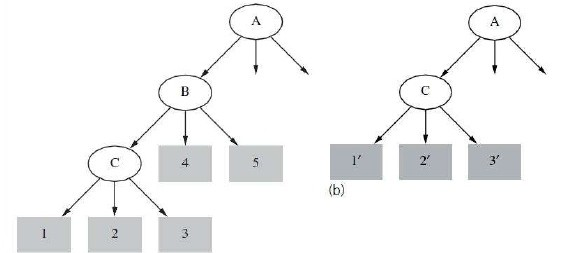
\includegraphics[scale=0.4]{DTreeStopping}
\end{column}
\end{columns}
\end{block}
\begin{block}{Results}
\begin{itemize}
\item Regret: my performance vs. best performance, averaged.
\end{itemize}
\begin{center}
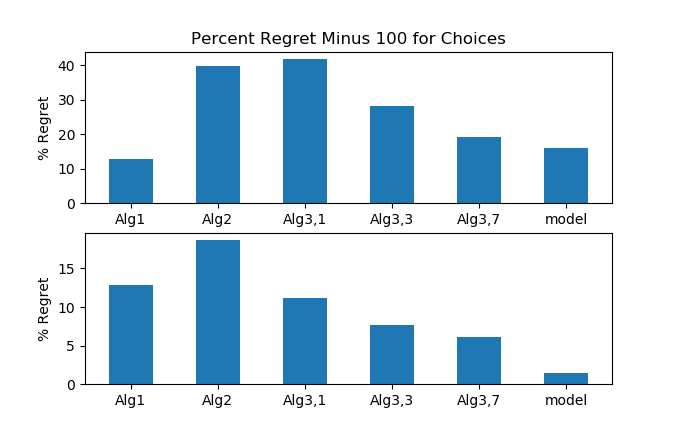
\includegraphics[scale=1.5]{Results}
\end{center}
\begin{itemize}
\item Does as well as Pythia~\cite{Kotsogiannis:2017} with same expressiveness as PINQ~\cite{McSherry:2010}.
\item Only as good as how well the programmer frames the ML problem.
\end{itemize}
\end{block}
\begin{block}{Bibliography}
\small{\bibliographystyle{unsrt}
\bibliography{Thesis}\vspace{0.75in}}
\end{block}
\end{column}
%\begin{column}{\sepwid}\end{column}
\end{columns}
\end{frame}
\end{document}